%%%%%%%%%%%%%%%%%%%%%%%%%%%%%%%%%%%%%%%
% A presentation by Gilles Bertrand   %
% GET/ ENST Bretagne - RSM department %
% gilles.bertrand at ieee dot org     %
% December 2006                       %
%%%%%%%%%%%%%%%%%%%%%%%%%%%%%%%%%%%%%%%

% Some options are passed here to allow the use of "cute" tables. See citation from "Beamer by example" below:
% "The first option, pdftex, provides
% information about the correct color driver to
% use. The option dvipsnames allows a set of predefined
% color names, such as RoyalBlue, to be used.
% (These named colors are sometimes referred to as
% the �Crayola� colors.) Finally, the table option
% informs xcolor that the colortbl package needs to
% be loaded."

\documentclass[pdf,xcolor=pdftex,dvipsnames,table]{beamer}

% The use of the university template is specified here
\usetheme{RWorkshop}

\usepackage{time}             % date and time
\usepackage{graphicx}
\usepackage[T1]{fontenc}      % european characters
%\usepackage{courier}
\usepackage{amssymb,amsmath}  % use mathematical symbols
\usepackage{bbding}           % special symbols like the heavy checkmark
\usepackage{palatino}					% use palatino as the default font
\setbeamercovered{transparent}

\hypersetup{% Set pdf properties
pdftitle = {A example presentation using beamer, QoS management in the IP Multimedia Subsystem},%
pdfauthor = {Gilles Bertrand},%
pdfsubject = {QoS in IMS},% 
pdfkeywords = {QoS, IMS, Policy, COPS},%
}

\begin{document}

% here you define the information that will be displayed in the title/cover page
\title[Intro to R Syntax]{\href{https://workrooms.ucalgary.ca/event/3768064}{Introduction to R Syntax}\footnote{Last generated:  \today ;  \now}\\}
\subtitle {Introduction to R Syntax as a key to language expression}
\author[Pablo Adames]{Pablo E Adames\\MEng, MSc, PEng\\
\vspace*{0.5cm}      	
%\includegraphics[height=0.5cm]{./figures/e-mail}
\href{mailto:pablo.adames@ucalgary.ca}{pablo.adames@ucalgary.ca}
}
\date{January 2$^\text{nd}$ and $3^\text{rd}$, 2024}


% this is used in the pdf information
%\subject{QoS management in the IP Multimedia Subsystem (IMS)}

% here you build the title page
\frame{
  \titlepage
}

% outline 
\AtBeginSection[]
{
  \begin{frame}
    \frametitle{Outline}
    \small
%    \tableofcontents[currentsection,hideothersubsections]
    \tableofcontents[currentsection]
    \normalsize
  \end{frame}
}
%

\section{Why Syntax?}
\begin{frame}
	\frametitle{What is the context for this workshop?}
	\begin{overprint}
	\onslide<1>{
			We engage in the following\ldots 
		\begin{itemize}
			\item Science/engineering
			\item Collecting data in experiments to  prove hypothesis
			\item Processing the data, concluding, communicating 
			\item Using computer tools to do all of these
	\end{itemize}	
	}
	\onslide<2->{
	\begin{itemize}
		\item Our tools are hardware and software
		\item Software lies on a spectrum:
	\end{itemize}
	}
	\visible<3->{
		\begin{center}
			\begin{figure}
				\scalebox{0.50}{
					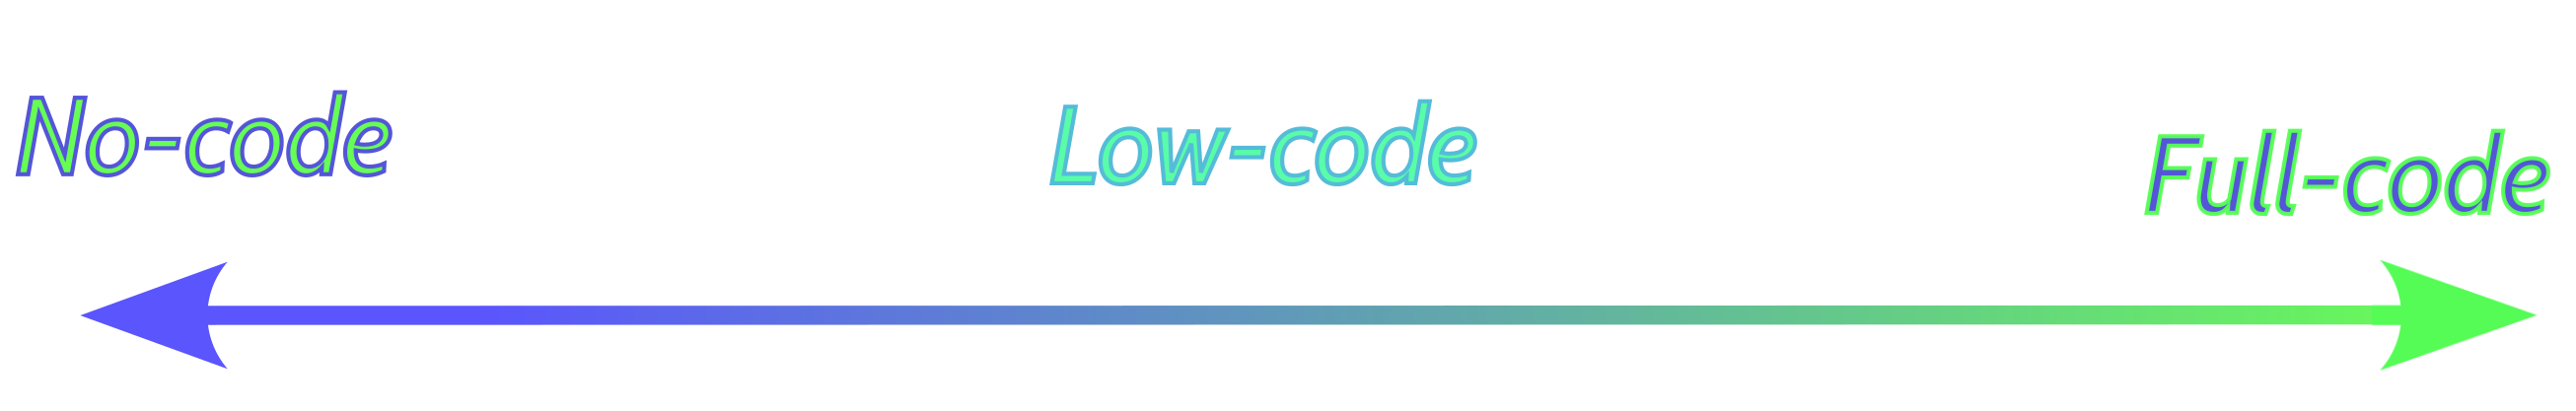
\includegraphics[scale=0.25]{./figures/Code_spectrum}
				}
			\end{figure}
		\end{center}
	}
	\end{overprint}
\end{frame}


\begin{frame}
	\frametitle{The tools for data processing}
	\begin{overprint}
		\onslide<1->{
			\begin{itemize}			
				\item Single-tier: own laptop/desktop/tablet and spreadsheets
				\item Multi-tier: remote server/computer clusters, database server, local programming editor and the terminal.
			\end{itemize}
		}
		\visible<2->{
			\begin{center}
				\begin{figure}
					\scalebox{0.50}{
						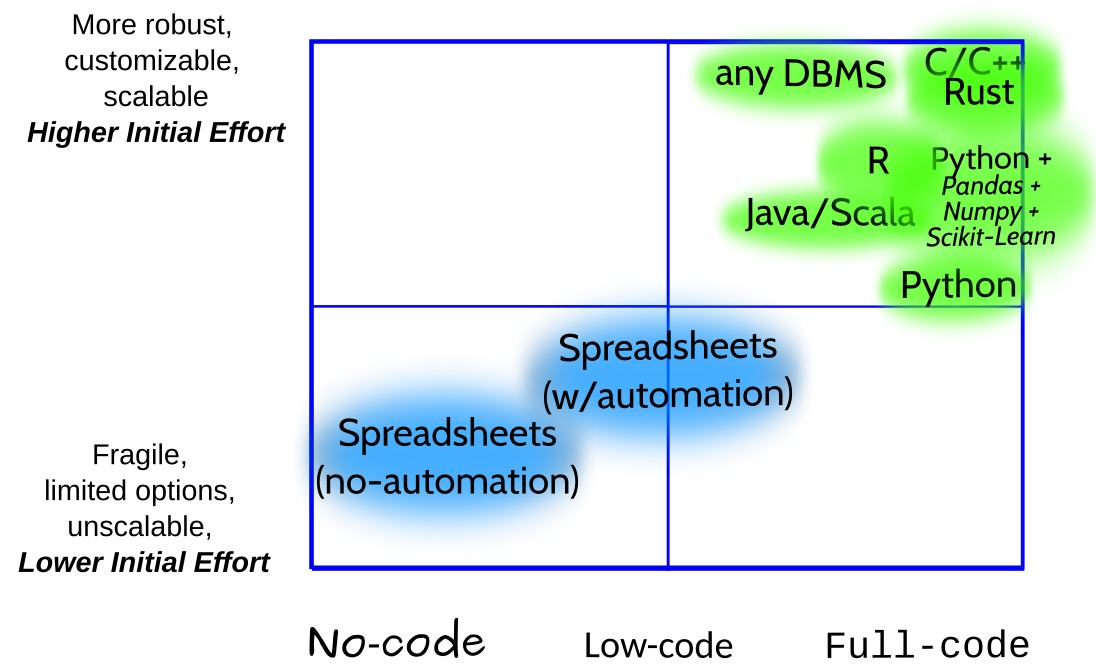
\includegraphics[scale=0.3]{./figures/EffortVsCode}
					}
					%\caption{Effort Vs. Code quadrants for data processing tools} 
				\end{figure}
			\end{center}
		}
		\visible<3->{
			\begin{itemize}
				\item[\CheckmarkBold] \textcolor{blue}{No silver bullet to do it all!}
				\item[\CheckmarkBold] \textcolor{blue}{Programming language(s) are essential}
			\end{itemize}
		}	   	
	\end{overprint}
\end{frame}


\begin{frame}
	\frametitle{Written language is a technology}
	\begin{overprint}
		\onslide<1>{
		\begin{itemize}
			\item Syntax is a key to unlock its power
			\item It's about how words get arranged to make sense to the receiver
		\end{itemize}
		}
		\onslide<2->{
			\begin{itemize}
				\item With the advent of Large Language Models (LLMs) 
				\item Some say ``computer programming is dead''
			\end{itemize}
		}
		\visible<3->{
			\vspace{0.5cm}
		\alert{This does not apply to you if\ldots}
		\begin{itemize}
			\item[\CheckmarkBold] \textcolor{blue}{You are (becoming) a career researcher}
			\item[\CheckmarkBold] \textcolor{blue}{You want to have precise control over the processing and visualization of your data} 
		\end{itemize}
		}
	\end{overprint}
\end{frame}


\begin{frame}
	\frametitle{General purpose Vs Data Processing Syntax}
	  \begin{block}{R is data oriented}
	    Statistical language, stats is about data and math. Its is natively vectorized and capable of graphics (no need of modules).   
  	\end{block}
  	\pause
	  \begin{block}{Systems-level languages}
	  	C/C++ and more recently Rust. They are used when real-time/high throughput is required
	  \end{block}
	  \pause
	  \begin{block}{General purpose languages}
	  	Java/Scala are JVM languages used heavily for distributed data processing (Spark framework). Python also falls into this category.
	  \end{block}
\end{frame}


\section{R syntax}


\begin{frame}
	\frametitle{Many R syntaxes}
	
	\begin{itemize}
		\item An R package can define its own syntax
		\item Three main-stream syntaxes in use
		\item They are equally valid ways of expression
	\end{itemize}
	\vspace{1cm}
	Excellent R syntax ``unofficial'' cheat sheet:

	{\footnotesize \textcolor{blue}{\url{https://github.com/rstudio/cheatsheets/blob/main/syntax.pdf}}}
	
\end{frame}


\begin{frame}
	\frametitle{Three main stream}
	\begin{overprint}
	\begin{columns}
		\column[c]{0.50\textwidth}
			\begin{itemize}
				\item<1,4> Dollar syntax or basic R syntax
				\item<2> Formula syntax, $y \sim x$
				\item<3> Tidyverse syntax, part of the \href{https://dplyr.tidyverse.org/}{dplyr grammar}
			\end{itemize}
		\column[c]{0.55\textwidth}
			\visible<1,4>{
				\begin{figure}
					\includegraphics[%trim=0 312 0 28,%
					% width=1\textwidth,%
					% height=0.70\textheight,
					%clip=true,%
					%keepaspectratio=true,%
					scale=0.21]%
					{./figures/R_Syntax_base_r}
				\end{figure}
			}
			\visible<2>{
				\begin{figure}
					\includegraphics[%trim=0 130 0 0,%
					% width=1\textwidth,%
					% height=0.70\textheight,
					%clip=true,%
					%keepaspectratio=true,%
					scale=0.21]%
					{./figures/R_Syntax_formula}
				\end{figure}
			}
			\visible<3>{
				\begin{figure}
					\includegraphics[%trim=0 312 0 28,%
					% width=1\textwidth,%
					% height=0.70\textheight,
					%clip=true,%
					%keepaspectratio=true,%
					scale=0.21]%
					{./figures/R_Syntax_tidyverse}
				\end{figure}
			}
	\end{columns}
	\end{overprint}
	\vspace{0.5cm}
	\visible<4>{We will focus on the base R syntax}

\end{frame}


\section{Basic concepts}
\subsection{Data representation}
\begin{frame}
	\frametitle{Data Representation}
	\begin{center}
	\begin{figure}
		\scalebox{0.90}{
			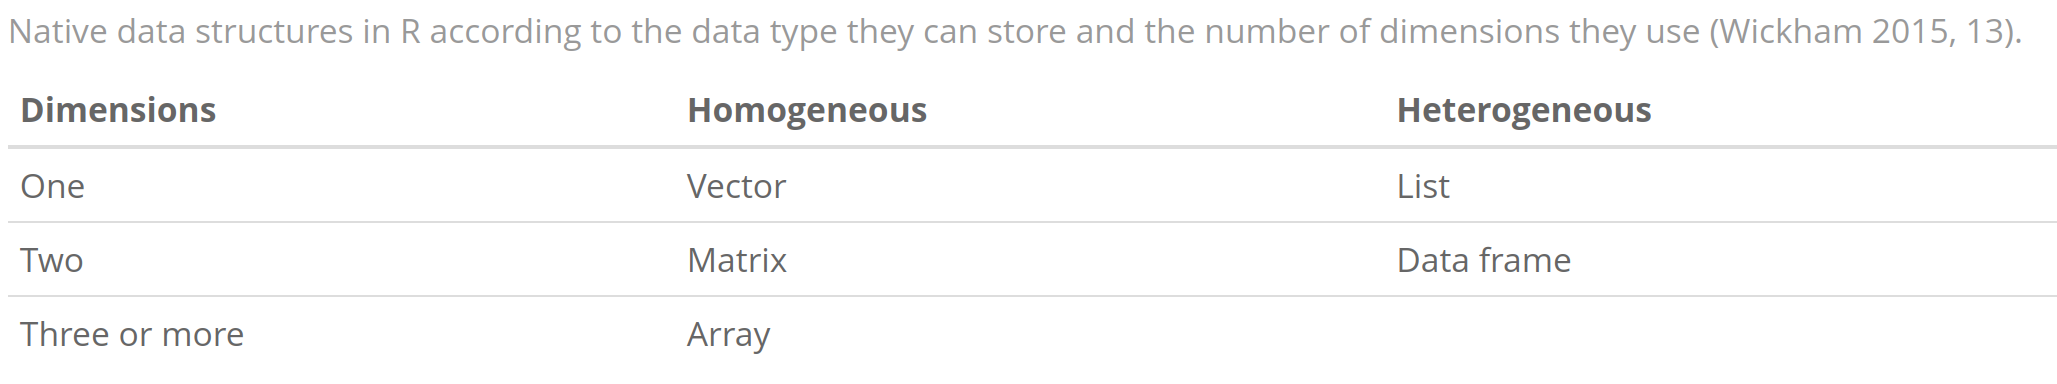
\includegraphics[scale=0.18]{./figures/Data_structures_table}
		} 
	\end{figure}
	\vspace{0.5cm}
	There are no scalars and everything is an object.
	\end{center}
\end{frame}


\subsection{Recycling}
\begin{frame}
	\frametitle{Recycling vectors}
	\begin{overprint}
	\begin{columns}
	\column{0.7\textwidth}
		\visible<1>{
			\begin{center}
				Element-wise multiplication
				\vspace{0.5cm}
				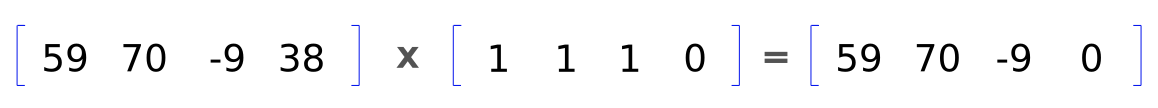
\includegraphics[scale=0.18]{./figures/vector_multiplication_base}	
			\end{center}
		}
		\visible<2,4>{
			\begin{center}
				Recycling a smaller vector
				\vspace{0.5cm}
					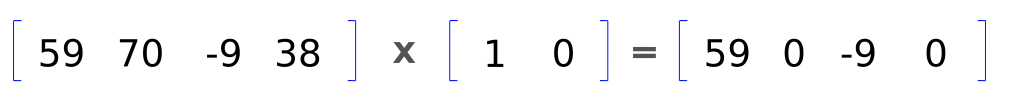
\includegraphics[scale=0.18]{./figures/vector_multiplication_recycle}	
			\end{center}
		}
		\visible<3>{
			\begin{center}
				Recycling explained\ldots
				
				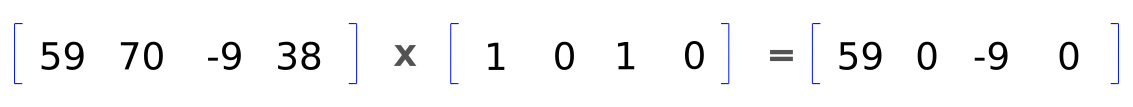
\includegraphics[scale=0.18]{./figures/vector_multiplication_recycle_expanded}	
			\end{center}
		}
		
	\column{0.3\textwidth}
	\visible<4>{
		\begin{center}
		\begin{figure}
			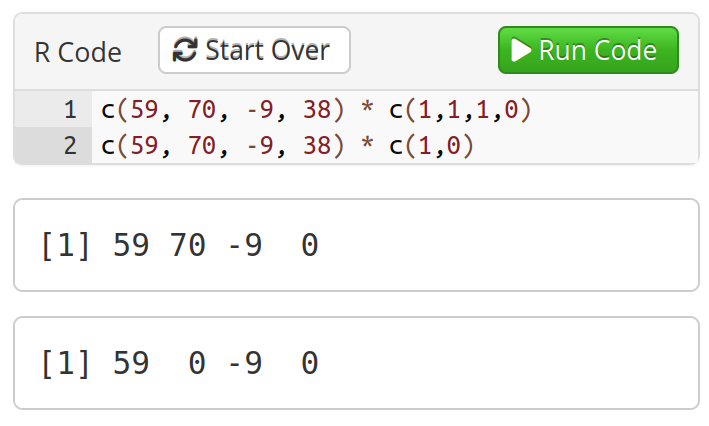
\includegraphics[scale=0.15]{./figures/Recycling_exaple_r_code} 
		\end{figure}
		\vspace{0.5cm}
		Recycling is a feature not a bug!
		\end{center}
	}
	\end{columns}
	\end{overprint}
\end{frame}

\subsection{Subsetting}
\begin{frame}
	\frametitle{Subsetting}
	\begin{center}
		\begin{figure}
			\scalebox{0.50}{
				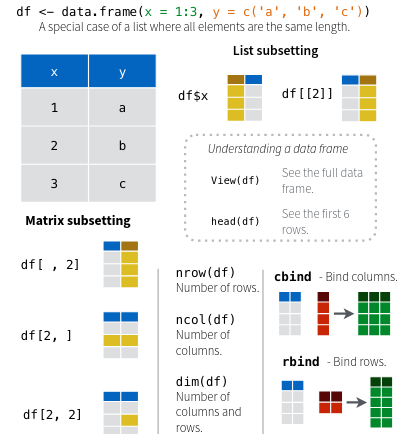
\includegraphics[scale=0.65]{./figures/Dataframe_shortcuts_from_BaseR_Cheat_Sheet}
			} 
		\end{figure}
		\vspace{0.5cm}
		This is native to the language, no need of libraries.
	\end{center}
\end{frame}



\section*{Thanking}
\begin{frame}
\frametitle{Thank you}
	
	\begin{block}{That was my last slide\ldots\\}
		\Large
		\emph{
			Now let's get to the workshop!
		}
		\normalsize
	\end{block}
\end{frame}

\section*{Bibliography}

\frame[allowframebreaks]
{
%  \frametitle{A (long) list of references}
  \nocite{*} % displays all references, cited or not
  \bibliographystyle{alpha}
  \footnotesize
  \bibliography{bibliography}
	\normalsize
}
\end{document}
